The top quark is one of the most interesting particles present in the Standard Model (SM) of
particle physics as it is postulated to interact with unknown particles from theories beyond the 
SM because of its high mass. Precise measurement of the properties of the top quark helps in the 
improvement of search sensitivity and test of perturbative Quantum Chromodynamics. Differential 
cross section measurements are used to test fixed-order predictions and extract QCD parameters. 
The \ttbar production is dominant at LHC and serves as the background for many new physics searches.

There have been many earlier measurements at 7, 8, and 13 \TeV center-of-mass energy 
as shown in Figure~\ref{fig:xss}. 
In this proceeding, we summarise the recent cross section measurements by the CMS experiment at the
LHC. For a more detailed description of each of the measurements, the reader is encouraged to look
at the corresponding paper. Here we summarise the \ttbar measurements in Section~\ref{sec:tt},
\tW in Section~\ref{sec:tW}, and $\ttbar$X in Section~\ref{sec:ttX} where X stands for 
\text{$\gamma$}, \cc, and \bb.

\begin{figure}[htb!]
\centering
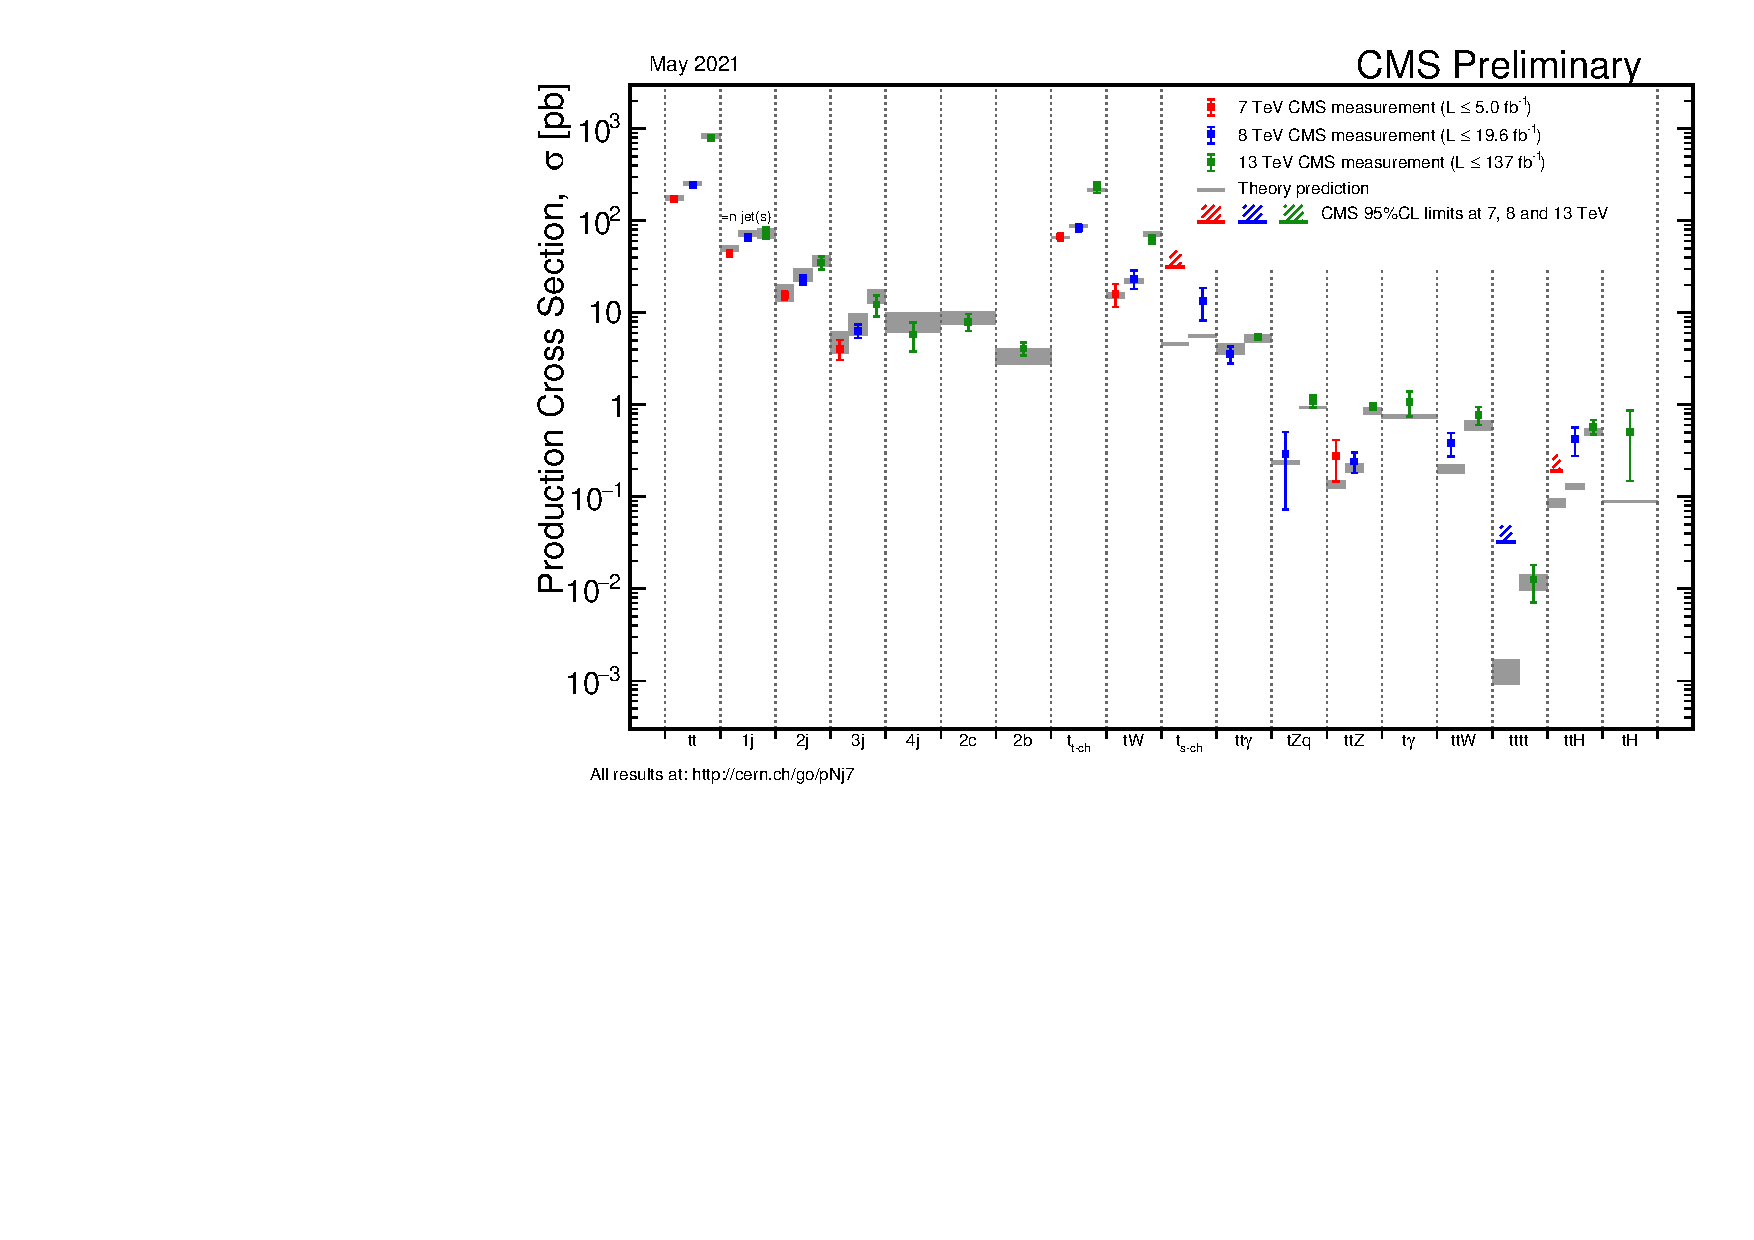
\includegraphics[width=1.0\linewidth]{SigmaNew_v8.pdf}
\caption{Top quark production cross section at various center-of-mass energies measured by the
	CMS experiment. The measurements are performed for the production of single \PQt, \ttbar, \ttbar + jets, \PQt + X, \ttbar+ X, \ttbar\ttbar, etc. Among these, a few of them are new at 13 \TeV whereas a
	few of them are still being studied. There is a good agreement between the predicted and
	measured values within the uncertainties.}
\label{fig:xss}
\end{figure}

